\documentclass[11pt,a4paper]{book}
\usepackage[english,greek]{babel}
\usepackage[utf8x]{inputenc}
\usepackage[noend]{algpseudocode}
\usepackage{algorithm}
\usepackage{amssymb,latexsym,amsmath,ucs,amsthm,setspace,graphicx,fancyvrb,float}
\usepackage{hyperref}
\usepackage{tkz-graph}
\usepackage{subfig}
\newtheorem*{lemma}{Λήμμα}
\newcommand{\HRule}{\rule{\linewidth}{0.5mm}}
\newcommand{\defeq}{\overset{\underset{\mathrm{def}}{}}{=}}
\makeatletter
\DeclareMathOperator*{\argmin}{arg\,min}
\makeatother
\raggedbottom
\begin{document}

\begin{titlepage}
\begin{center}


\includegraphics[width=0.15\textwidth]{Pyrforos3.png}\\[1cm]
\textsc{\LARGE Εθνικό Μετσόβιο Πολυτεχνείο}\\[1.5cm]

\Large{ 3η Γραπτή Άσκηση }\\[0.5cm]

% Title
\begin{doublespace}
\HRule \\[0.4cm]
{\huge \bfseries
Αλγόριθμοι \& Πολυπλοκότητα
}\\[0.4cm]
\end{doublespace}

\HRule \\[1.5cm]

\begin{minipage}{0.4\textwidth}
\begin{flushleft} \large
\emph{Σπουδαστής:} \\
Διονύσης \textsc{Ζήνδρος} (06601)\\
\textlatin{\textless dionyziz@gmail.com\textgreater}
\end{flushleft}
\end{minipage}
\begin{minipage}{0.4\textwidth}
\begin{flushright} \large
\emph{Διδάσκοντες:} \\
Στάθης \textsc{Ζάχος}\\
Δημήτρης \textsc{Φωτάκης}
\end{flushright}
\end{minipage}

\vfill

{\large 24 Ιανουαρίου 2011}
\end{center}
\end{titlepage}

\section*{Άσκηση 1}
\section*{Άσκηση 2}
\section*{Άσκηση 3}
\section*{Άσκηση 4}
\subsection*{(α)}

Ο ακόλουθος γράφος έχει μοναδικό ΕΣΔ, αλλά περιέχει ακμές ίδιου βάρους:

\selectlanguage{english}
\begin{figure}[ht]
	\centering
		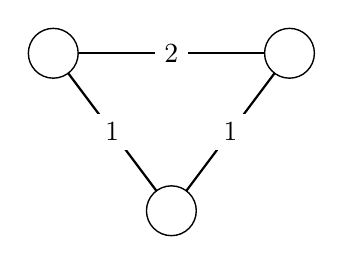
\begin{tikzpicture}
			\Vertex[x=0,y=0,L=\ ]{1}
			\Vertex[x=3,y=0,L=\ ]{2}
			\Vertex[x=1.5,y=-2,L=\ ]{3}

			\Edge[label=2](1)(2)
			\Edge[label=1](1)(3)
			\Edge[label=1](2)(3)
		\end{tikzpicture}
\end{figure}
\selectlanguage{greek}

\subsection*{(β)}
Ο γράφος του υποερωτήματος (α) έχει μοναδικό ΕΣΔ αλλά περιέχει ακμές ίδιου βάρους που είναι οι ελάχιστες που διασχίζουν την ίδια τομή.

\begin{lemma}
Κάθε ακμή ενός ΕΣΔ ενός συνεκτικού μη κατευθυνόμενου ζυγισμένου γράφου είναι η ελάχιστη που διασχίζει κάποιο κόψιμο.
\end{lemma}
\begin{proof}
Έστω τέτοιος γράφος $G = (V, E, w)$ με ένα ΕΣΔ του $T \subseteq E$ και έστω ότι υπάρχει κάποια ακμή $e = (u, v) \in T$ τέτοια ώστε να μην υπάρχει κόψιμο του G το οποίο να είναι η ελάχιστη που το διασχίζει. Τότε έστω $K$ το ΕΣΔ που κατασκευάζει ο αλγόριθμος του \textlatin{Kruskal}. Κατά την εκτέλεση του αλγορίθμου, υπάρχει κάποιο βήμα κατά το οποίο γίνεται ένωση των ανεξάρτητων συνόλων που περιέχουν τους κόμβους $u$ και $v$ μέσω κάποιας ακμής $f$ η οποία είναι ελάχιστη σε ένα κόψιμο το οποίο διασχίζει και η $e$ και άρα $w(f) < w(e)$. Όμως στο $T$ η ακμή $e$ μπορεί να αντικατασταθεί από την $f$ και το δέντρο να παραμείνει συνεκτικό και με βάρος $w( T \cup \{f\} \setminus \{e\}) < w( T )$. Άρα το $T$ δεν είναι ΕΣΔ, κάτι το οποίο αποτελεί αντίφαση.
\end{proof}

\begin{lemma}
Κάθε συνεκτικός μη κατευθυνόμενος ζυγισμένος γράφος στον οποίο για κάθε τομή η ακμή ελάχιστου βάρους που τη διασχίζει είναι μοναδική έχει μοναδικό ΕΣΔ.
\end{lemma}
\begin{proof}
Έστω τέτοιος γράφος $G = (V, E, w)$ και δύο ΕΣΔ του, $Τ \subseteq E$ και $T' \subseteq E$,
με $T \neq T'$ και $w(T) = w(T')$.

Τότε, επειδή $T \neq T$, θα υπάρχει κάποια ακμή $e = (u, v)$ με $e \in T \land e \not\in T'$. Από το παραπάνω λήμμα, η $e$ θα είναι η ελάχιστη που διασχίζει κάποιο κόψιμο του $T$, έστω $S$.

Τώρα, επειδή το $T'$ είναι συνεκτικό δέντρο, θα υπάρχει μοναδικό μονοπάτι από τον κόμβο $u$ στον κόμβο $v$ που διασχίζει το $S$ με κάποια ακμή, έστω $e' \neq e$. Αφού $w(e) < w(e')$, αντικαθιστώντας την ακμή $e'$ με την $e$ στο $T'$ παίρνουμε ένα συνεκτικό δέντρο με βάρος $w(T' \cup\{e\} \setminus \{e'\}) < w(T')$. Άρα το $T'$ δεν είναι ελάχιστο συνεκτικό δέντρο, κάτι το οποίο αποτελεί αντίφαση.

Άρα το ΕΣΔ είναι μοναδικό.
\end{proof}

\subsection*{(γ)}
\subsection*{(δ)}

\section*{Άσκηση 5}
\subsection*{(α)}
\begin{lemma}
Σε ένα συνεκτικό κατευθυνόμενο ζυγισμένο γράφο, για κάθε κύκλο υπάρχει ΕΣΔ που δεν περιέχει την ακμή μέγιστου βάρους του κύκλου αυτού.
\end{lemma}

\begin{proof}
Έστω τέτοιος γράφος $G = (V, E, w)$ με κάποιον κύκλο $C$ και έστω ένα ΕΣΔ $T \subseteq E$ που περιέχει την ακμή $e$ μέγιστου βάρους του $C$. Τότε έστω το δάσος $T \setminus \{ e \}$ που θα αποτελείται από δύο συνδεδεμένους υπογράφους. Θα υπάρχει μία ακμή $f \in E$ που θα συνδέει αυτούς τους δύο συνδεδεμένους υπογράφους με $f \neq e$ και άρα $w( f ) \leq w( e )$. Αντικαθιστώντας την $e$ με την $f$ στο $T$ προκύπτει ένα συνεκτικό δέντρο με βάρος $w( T \cup \{ f \} \setminus \{ e \} ) \leq w( T )$. Άρα το $T \cup \{ f \} \setminus \{ e \}$ είναι ΕΣΔ.
\end{proof}

\subsection*{(β)}
\subsection*{(γ)}

\end{document}
